%% LyX 2.3.0 created this file.  For more info, see http://www.lyx.org/.
%% Do not edit unless you really know what you are doing.
\documentclass[english]{beamer}
\usepackage{natbib}
\usepackage{mathptmx}
\usepackage[T1]{fontenc}
\usepackage[latin9]{inputenc}
\usepackage{wrapfig}
\usepackage{amsmath}
\usepackage{amssymb}
\usepackage{graphicx}

\makeatletter

%%%%%%%%%%%%%%%%%%%%%%%%%%%%%% Textclass specific LaTeX commands.
% this default might be overridden by plain title style
\newcommand\makebeamertitle{\frame{\maketitle}}%
% (ERT) argument for the TOC
%\AtBeginDocument{%
%  \let\origtableofcontents=\tableofcontents
%  
%\def\tableofcontents{\@ifnextchar[{\origtableofcontents}{\gobbletableofcontents}}
%  \def\gobbletableofcontents#1{\origtableofcontents}
%}

%%%%%%%%%%%%%%%%%%%%%%%%%%%%%% User specified LaTeX commands.
%\usetheme{Warsaw}
% or ...

%\setbeamercovered{transparent}
% or whatever (possibly just delete it)

\makeatother

\usepackage{babel}
\begin{document}

\title{Hypercoercions and a Framework for Equivalence of Cast Calculi}

\author{Kuang-Chen Lu\inst{1} \and Jeremy G. Siek\inst{1}\and Andre Kuhlenschmidt\inst{1}}

\institute{\inst{1}Department of Computer Science\\
Indiana University Bloomington}

\date[WGT 2003]{Workshop on Gradual Typing, 2020}

\makebeamertitle

\pgfdeclareimage[height=0.5cm]{institution-logo}{institution-logo.jpg}
\logo{\pgfuseimage{institution-logo}}

%\AtBeginSubsection[]{%
%  \frame<beamer>{ 
%    \frametitle{Outline}   
%    \tableofcontents[currentsection,currentsubsection] 
%  }
%}

%\beamerdefaultoverlayspecification{<+->}
\begin{frame}{Outline}

\tableofcontents{}

\end{frame}

\section{Hypercoercions}

\subsection{The Space-Efficiency Problem}
\begin{frame}{An Example Program}

\framesubtitle{}

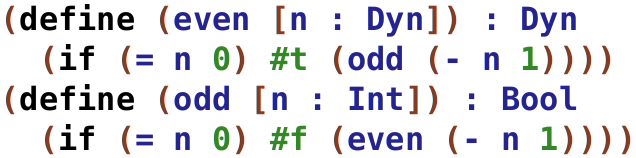
\includegraphics[scale=0.3]{resources/even-odd}
\end{frame}
%
\begin{frame}{The Space-Efficiency Problem}
\begin{itemize}
\item Casts might accumulate on continuations (call stacks)
\item Casts might accumulate in values as proxies
\end{itemize}
\end{frame}
%

\subsection{Existing Solutions}
\begin{frame}{Solutions: Space-Efficient Cast Representations}

\begin{itemize}
\item Coercions in normal forms \cite{herman2010space,siek2012interpretations,Siek:2015:BCT:2737924.2737968}
\item Threesomes \cite{Siek:2010:TWB:1706299.1706342,Garcia:2013:CTB:2500365.2500603}
\item Supercoercions \cite{Garcia:2013:CTB:2500365.2500603}
\end{itemize}
\end{frame}
%
\begin{frame}{Criteria for ``Good'' Cast Representations }

\begin{figure}
\begin{minipage}[t]{0.45\textwidth}%

\includegraphics[scale=0.25]{resources/thinking-face}%
\end{minipage}\hfill{}%
\begin{minipage}[t]{0.45\textwidth}%
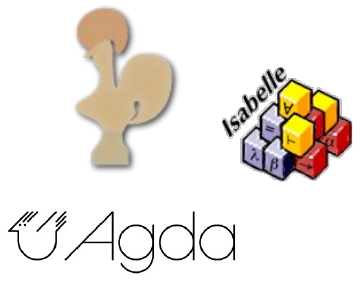
\includegraphics[scale=0.5]{resources/all-proof-assistants}%
\end{minipage}
\end{figure}
\end{frame}
%
\begin{frame}{Threesomes are Difficult to Understand}

\begin{figure}
\noindent\begin{minipage}[t][1\totalheight][c]{1\columnwidth}%
\begin{wrapfigure}{I}{0.5\columnwidth}%
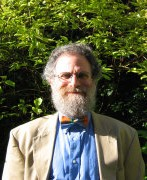
\includegraphics[scale=0.7]{resources/Philip_Wadler}\end{wrapfigure}%
\textit{``\ldots{} while preparing a lecture on threesomes a few years
after the paper was published, he required several hours to puzzle
out the meaning of his own notation, $\bot^{mGp}$''\cite{Siek:2015:BCT:2737924.2737968}}%
\end{minipage}
\end{figure}
\end{frame}
%
\begin{frame}{Coercions in Normal Form are Difficult to Mechanize}

\begin{figure}
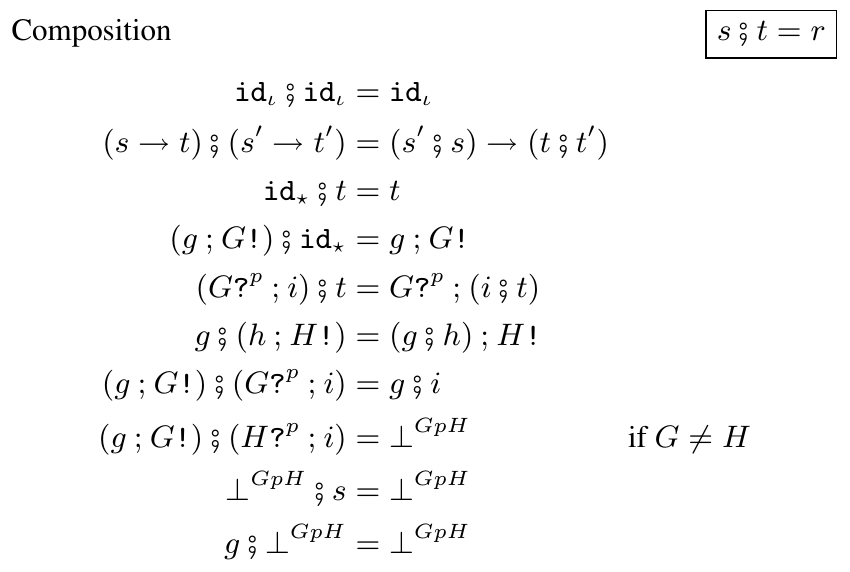
\includegraphics[scale=0.3]{resources/composition-of-coercions-in-normal-form} 

v.s. 

\textasciitilde 100 Lines of Agda Code
\end{figure}
\end{frame}
%

\subsection{Our Solution: Hypercoercions}
\begin{frame}{Our Solution: Hypercoercions}

\begin{figure}
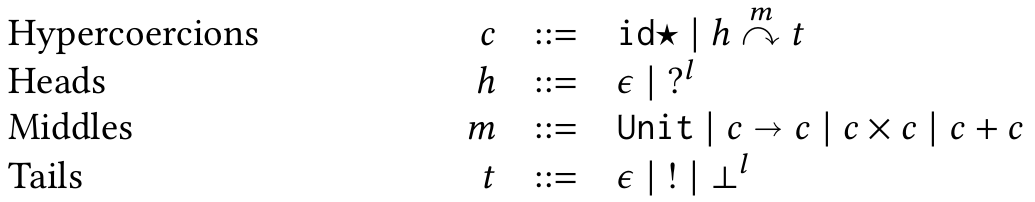
\includegraphics[scale=0.4]{resources/hypercoercions-syntax}

Composition of hypercoercions is morally a structural recursion!
\end{figure}
\end{frame}

\section{Equivalence of Cast Calculi}

\subsection{Cast Representations Should be Proved Correct}
\begin{frame}{What do We Mean by a Cast Representation is Correct?}

\[
\text{eval}_{X}(e)=o\text{ if and only if }\text{eval}_{\text{D}}(e)=o
\]

\[
\text{eval}_{X}(e)=o\text{ if and only if }\text{eval}_{\text{UD}}(e)=o
\]
\end{frame}
%

\subsection{Our Solution: CastADT + Parameterized Dynamics}
\begin{frame}{Our Solution: Every Lazy D CastADT is Correct}
\begin{theorem}
Suppose that $C$ is a Lazy D Cast ADT. If $e:T$ and $o:T$ then
\[
\text{eval}_{S(C)}(e)=o\text{ if and only if }\text{eval}_{\text{D}}(e)=o
\]
\end{theorem}

\end{frame}
%
\begin{frame}{How does $S(C)$ work?}
\begin{itemize}
\item Every continuation has exactly one cast frame at the top.
\item Every non-constant value has exactly one proxy.
\end{itemize}
\end{frame}
%
\begin{frame}{What is a Cast ADT?}

\begin{table}
\begin{tabular}{rl}
$\text{id}(T)=c$ & identity cast\tabularnewline
$\text{seq(c,c)}=c$ & cast composition\tabularnewline
$\text{cast}(T,l,T)=c$ & translate casts in source language\tabularnewline
$\text{applyCast}(v,c)=r$ & cast application\tabularnewline
\end{tabular}
\end{table}
\end{frame}
%
\begin{frame}{What is a Lazy D Cast ADT?}
\begin{itemize}
\item $\text{applyCast}(\text{id}(T),v)=\text{succ}(v)$
\item $\text{applyCast}(\text{seq}(c,d),v)=\text{applyCast}(c,v)\underline{\gg}\lambda u.\text{applyCast}(d,u)$
\item $\text{applyCast}(\text{cast}(S,l,T),v)$ respects the Lazy D blame
strategy.
\end{itemize}
\end{frame}

\section*{Summary}
\begin{frame}{Summary}
\begin{itemize}
\item We presented Lazy D and Lazy UD \alert{hypercoercions}.
\item We proved that every \alert{Lazy D Cast ADT} is correct.
\end{itemize}
\medskip{}

\begin{itemize}
\item Outlook
\begin{itemize}
\item Define a Lazy UD Cast ADT and prove a similar theorem.
\item Prove existing cast representations are Lazy D/UD Cast ADT
\end{itemize}
\end{itemize}
\end{frame}
%
\begin{frame}{References}

\bibliographystyle{plain}
\bibliography{/home/lukc/hypercoercion-and-framework-wgt2020/bibfile}
\end{frame}

\end{document}
